% !Mode:: "TeX:UTF-8"
%!TEX program  = xelatex

\documentclass{cumcmthesis}
%\documentclass[withoutpreface,bwprint]{cumcmthesis} %去掉封面与编号页
%\documentclass[UTF8]{ctexart} 
%\setlength\parindent{2em}
\usepackage{url}
\usepackage{array}
\usepackage{amsmath} 
\usepackage{amssymb}
\usepackage{amsfonts}
\usepackage{caption}
\usepackage{booktabs}
\usepackage{color}
\usepackage{enumerate}
\usepackage{xpatch}
\usepackage{graphicx}
\usepackage{longtable}
\usepackage{multirow}
\usepackage{comment}
\usepackage{subfigure}
\usepackage{supertabular}
\usepackage{floatrow}
\usepackage{cite}
\usepackage{float}
\xpatchcmd{\thebibliography}{\section*}{\section}{}{}
%\newcommand{\upcite}[1]{\textsuperscript{\textsuperscript{\cite{#1}}}}

\title{装箱问题}
\tihao{A}
\baominghao{201922002029}
\schoolname{重庆邮电大学}
\membera{陈恒宇}
\memberb{邓韦}
\memberc{殷寰宇}
\supervisor{虞继敏}
\yearinput{2019}
\monthinput{09}
\dayinput{15}


\begin{document}
\maketitle
\begin{abstract}
        本文通过

        针对问题一,
        
        针对问题二,
        
        针对问题三,
        
        针对问题四,
        
\keywords{关键词}
\end{abstract}
%\thispagestyle{empty}

%目录
\tableofcontents
%\thispagestyle{empty}

\newpage

\section{问题重述}

\subsection{问题背景}
              

\subsection{问题的提出}
    
        根据……,
    建立数学模型回答以下问题:
\begin{itemize}
    \item[1)]
    \item[2)]
    \item[3)]
    \item[4)]
\end{itemize}

\section{问题分析}
\subsection{问题一的分析}   


\subsection{问题二的分析}
        

\subsection{问题三的分析}
        

\subsection{问题四的分析}
     

\section{基本假设}
    

\section{符号说明}
\begin{center}
\begin{tabular}{ccc}
%\caption[table]{符号说明}
\toprule[2pt]
\makebox[0.2\textwidth][c]{符号}&\makebox[0.5\textwidth][c]{意义}&\makebox[0.2\textwidth][c]{单位} \\
\midrule[1pt]
 $R_i$  &  第$i$个雷达  & / \\ 
 $r_i$  &  飞行物与第$i$个雷达之间距离的观测值  &  米  \\ 
 $(x_i,y_i,z_i)$  &  第$i$个雷达的坐标  &  米  \\ %\hline
 $S(x,y,z)$  &  飞行物坐标  &  米  \\% \hline
 $N$  &  飞行物乙的$x$轴坐标  &  公里 \\ %\hline
 $M$  &  安全区的$y$轴坐标  &  公里  \\
 $h$  &  飞行物乙的$z$轴坐标  &  公里  \\
 $V$  &  敌机的飞行速度  &  马赫数  \\
 $U$  &  I型追踪导弹的速度  &  马赫数  \\
 $V_{\text{声}}$  &  测量地的音速  &  米/秒  \\
 $n$  &  雷达的个数  &  个  \\
\bottomrule[1.5pt]
\end{tabular}
\end{center}

\section{问题一的求解}

\subsection{问题一的分析}

\subsection{模型的求解}

\section{问题二的求解}

\subsection{问题二的分析}

\subsection{模型的建立与求解}


\section{问题三的求解}

\subsection{问题三的分析}


\subsection{模型的建立与求解}


\section{问题四的求解}

\subsection{问题四的分析}
        

\subsection{模型的建立与求解}


\section{灵敏度检验}

\section{模型的评价和推广}
\subsection{模型的评价}
\subsubsection{模型的优点}

\subsubsection{模型的缺点}
   

%参考文献
\begin{thebibliography}{9}%宽度9
\bibitem{bib:one}曾文军,曾小雨,郑娟,朱金伟.
    多雷达定位误差简析[J].高等函授学报(自然科学版),
    2008(05):57-59.
\bibitem{bib:two}

\end{thebibliography}


\newpage
%附录
\begin{appendices}
\section{引用}
  问题一要求我们根据CMA热带气旋最佳路径数据集和其他相关资料,
对中国各省(以地级市为单位)进行热带气旋的风险评估。
首先统计出1949年-2018年登录我国沿海各省份的热带气旋数量,
并选取其中登录次数最多的四个省份作为评估对象。
其次确定评定热带气旋风险等级的八个因素:受热带气旋影响过程中的
平均降雨量、日最大降雨量、平均风速、日最低气压、热带气旋的登陆频次、持续时间、
造成的人员伤亡数和直接经济损失。
接着确定四个热带气旋风险等级分别为:灾情较轻,灾情一般,灾情较重,灾情严重。
由于对热带气旋风险的评估属于模糊决策,故采用模糊综合评价法求出各省受热带气旋
影响的评价结果。\cite{bib:one}
最后在四个受灾最严重的省份中各选取四个典型城市,采用相同的方法进行风险评估,
并结合地理、气候因素分析其对风险等级的影响。

\section{排队算法--matlab 源程序}
    \begin{lstlisting}[language=matlab]
    kk=2;[mdd,ndd]=size(dd);
    while ~isempty(V)
    [tmpd,j]=min(W(i,V));tmpj=V(j);
    for k=2:ndd
    [tmp1,jj]=min(dd(1,k)+W(dd(2,k),V));
    tmp2=V(jj);tt(k-1,:)=[tmp1,tmp2,jj];
    end
    tmp=[tmpd,tmpj,j;tt];[tmp3,tmp4]=min(tmp(:,1));
    if tmp3==tmpd, ss(1:2,kk)=[i;tmp(tmp4,2)];
    else,tmp5=find(ss(:,tmp4)~=0);tmp6=length(tmp5);
    if dd(2,tmp4)==ss(tmp6,tmp4)
    ss(1:tmp6+1,kk)=[ss(tmp5,tmp4);tmp(tmp4,2)];
    else, ss(1:3,kk)=[i;dd(2,tmp4);tmp(tmp4,2)];
    end;end
    dd=[dd,[tmp3;tmp(tmp4,2)]];V(tmp(tmp4,3))=[];
    [mdd,ndd]=size(dd);kk=kk+1;
    end; S=ss; D=dd(1,:);
    \end{lstlisting}

\section{长表格}
\begin{longtable}[c]{p{0.2\textwidth}<{\centering}|p{0.1\textwidth}<{\centering}p{0.2\textwidth}<{\centering}}
    %\centering
    \caption{abcd} \\
    \toprule[2pt]
    增益介质&功率& 波长\\ 
    \midrule[1pt]
    \endfirsthead
    \caption[]{abcd(绪)} \\
    %\multicolumn{3}{r}{\footnotesize 接上页} \\ 
    \toprule[2pt]
    增益介质&功率&波长\\ 
    \midrule[1pt]
    \endhead
    \bottomrule[1.5pt] 
    %\multicolumn{3}{r}{\footnotesize 接下页} \\
    \endfoot
    \bottomrule[1.5pt]
    \endlastfoot
    HeNe & \multicolumn{2}{c}{000} \\
    HeNe & 1mW & 633nm \\\cline{1-2} 
    %纵向合并
    \multirow{2}{0.2\textwidth}{\centering000}
     & 1mW & 633nm \\
     & 1mW & 633nm \\
    HeNe & 1mW & 633nm \\
    HeNe & 1mW & 633nm \\
    HeNe & 1mW &  633nm \\
    HeNe & 1mW & 633nm \\
    HeNe & 1mW & 633nm \\
    HeNe & 1mW & 633nm \\
    HeNe & 1mW & 633nm \\
    HeNe & 1mW & 633nm \\
    HeNe & 1mW & 633nm \\
    HeNe & 1mW & 633nm \\
    HeNe & 1mW & 633nm \\
    HeNe & 1mW & 633nm \\
    HeNe & 1mW & 633nm \\
    HeNe & 1mW & 633nm \\
    HeNe & 1mW & 633nm \\
    HeNe & 1mW & 633nm \\
    HeNe & 1mW & 633nm \\
    HeNe & 1mW & 633nm \\
    HeNe & 1mW & 633nm \\
    HeNe & 1mW & 633nm \\
    HeNe & 1mW & 633nm \\
    HeNe & 1mW & 633nm \\
    HeNe & 1mW & 633nm \\
    HeNe & 1mW & 633nm \\
    HeNe & 1mW & 633nm \\
    HeNe & 1mW & 633nm \\
    HeNe & 1mW & 633nm \\
    HeNe & 1mW & 633nm \\
    HeNe & 1mW & 633nm \\
    HeNe & 1mW & 633nm \\
\end{longtable}

\section{表格}
\begin{table}[htbp]
    \caption{风险评估对象(地级市)}
    \centering    
    \label{table1}
    \begin{tabular}{m{0.1\textwidth}<{\centering}|
        m{0.1\textwidth}<{\centering}m{0.1\textwidth}<{\centering}
        m{0.1\textwidth}<{\centering}m{0.1\textwidth}<{\centering}}
    \toprule[2pt]
         省份  &  \multicolumn{4}{c}{城市}  \\%横向合并
    \midrule[1pt]
        浙江  &  杭州  &  湖州  &  金华  &  丽水  \\
        \cline{1-3}
        %纵向合并
        \multirow{3}{0.1\textwidth}{福建广东海南}
        &  福州  &  厦门  &  宁德  &  福鼎  \\
        &  徐闻  &  广州  &  汕头  \vline&  湛江  \\
        &  三亚  &  东方  &  儋县  &  海口  \\
        %\renewcommand{\arraystretch}{1.5}行距加宽50% 
    \bottomrule[1.5pt]
    \end{tabular}
\end{table}

\section{图片}
\begin{figure}[!h]
    \centering
    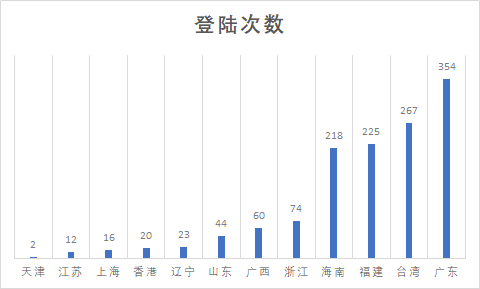
\includegraphics[width=.6\textwidth]{1949-2018_province_occurence.png}
    \caption{1949年到2018年我国沿海各省份热带气旋的登陆次数柱状图}
    \label{figure1}
\end{figure}


\section{并排图片、表格}
\begin{figure}[H]
    \begin{floatrow} \CenterFloatBoxes
    \ffigbox{\caption{2}}{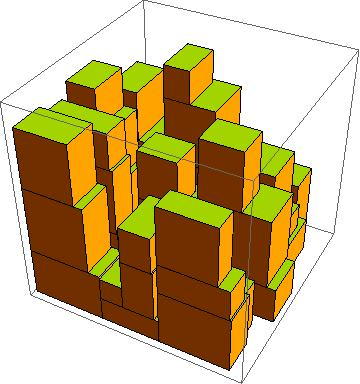
\includegraphics[width=.3\textwidth]{2.jpg}}
    \killfloatstyle
    \ttabbox{\caption{3}}{
    \begin{tabular}{|m{0.1\textwidth}<{\centering}|m{0.1\textwidth}<{\centering}|m{0.1\textwidth}<{\centering}|}\hline
        a & b & c \\ \hline
        1 & 2 & 3 \\ \hline
    \end{tabular}}
\end{floatrow}
\end{figure}

\begin{figure}[H]
    \begin{floatrow}
    \ffigbox{\caption{1}}{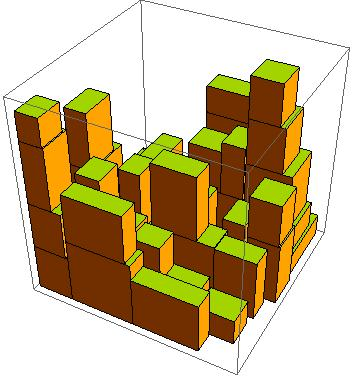
\includegraphics[width=.3\textwidth]{1.jpg}}
    \ffigbox{\caption{2}}{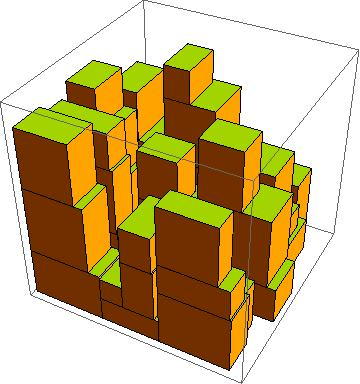
\includegraphics[width=.3\textwidth]{2.jpg}}
\end{floatrow}
\end{figure}

\section{数学公式}
\begin{equation}
    \sum\limits_{n=1}^Na_n
\end{equation}


\begin{equation}
    \begin{matrix} 
        r_{11}  &&    \cdots  &&  r_{1n}  \\
        r_{21}  &&  \cdots  &&  r_{2n}    \\ 
        \cdots  &&  \cdots  &&  \cdots    \\
        r_{81}  &&  \cdots  &&  r_{8n}    \\ 
    \end{matrix} 
    \quad\quad
    \begin{pmatrix} 
        r_{11}  &&  \cdots  &&  r_{1n}  \\
        r_{21}  &&  \cdots  &&  r_{2n}  \\ 
        \cdots  &&  \cdots  &&  \cdots  \\
        r_{81}  &&  \cdots  &&  r_{8n}  \\ 
    \end{pmatrix} 
    \quad\quad
    \begin{bmatrix} 
        r_{11}  &&  \cdots  &&  r_{1n}  \\
        r_{21}  &&  \cdots  &&  r_{2n}  \\ 
        \cdots  &&  \cdots  &&  \cdots  \\
        r_{81}  &&  \cdots  &&  r_{8n}  
    \end{bmatrix} 
\end{equation}

\begin{equation}
    \begin{Bmatrix} 
        r_{11}  &&  \cdots  &&  r_{1n}  \\
        r_{21}  &&  \cdots  &&  r_{2n}  \\ 
        \cdots  &&  \cdots  &&  \cdots  \\
        r_{81}  &&  \cdots  &&  r_{8n}  \\
    \end{Bmatrix} 
    \quad\quad
    \begin{vmatrix} 
        r_{11}  &&  \cdots  &&  r_{1n}  \\
        r_{21}  &&  \cdots  &&  r_{2n}  \\ 
        \cdots  &&  \cdots  &&  \cdots  \\
        r_{81}  &&  \cdots  &&  r_{8n}  \\
    \end{vmatrix} 
    \quad\quad
    \begin{Vmatrix} 
        r_{11}  &&  \cdots  &&  r_{1n}  \\
        r_{21}  &&  \cdots  &&  r_{2n}  \\ 
        \cdots  &&  \cdots  &&  \cdots  \\
        r_{81}  &&  \cdots  &&  r_{8n}  
    \end{Vmatrix}     
\end{equation}



\end{appendices}
\end{document} 

%编号
%\begin{itemize}
    %\item[1)]
    %\item[2)]
    %\item[3)]
    %\item[4)]
%\end{itemize}


%表格
%\begin{table}[htbp]
    %\centering
    %\caption{风险评估对象(地级市)}
    %\label{table1}
    %\begin{tabular}{p{0.1\textwidth}<{\centering}|
    %    p{0.1\textwidth}<{\centering}p{0.1\textwidth}<{\centering}
    %    p{0.1\textwidth}<{\centering}p{0.1\textwidth}<{\centering}}
    %\toprule[2pt]
    %     省份  &  \multicolumn{4}{c}{城市}  \\
    %\midrule[1pt]
    %    浙江  &  杭州  &  湖州  &  金华  &  丽水  \\
    %    福建  &  福州  &  厦门  &  宁德  &  福鼎  \\
    %    广东  &  徐闻  &  广州  &  汕头  &  湛江  \\
    %    海南  &  三亚  &  东方  &  儋县  &  海口  \\
    %\bottomrule[1.5pt]
    %\end{tabular}
%\end{table}

%图
%\begin{figure}[!h]
    %\centering
    %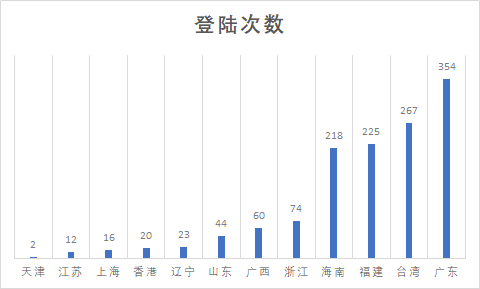
\includegraphics[width=.6\textwidth]{1949-2018_province_occurence.png}
    %\caption{1949年到2018年我国沿海各省份热带气旋的登陆次数柱状图}
    %\label{figure1}
%\end{figure}

%矩阵
%\begin{equation}
    %\begin{bmatrix} 
        % R_1  \\
        % R_2  \\
        % \cdots  \\
        % R_n   
    %\end{bmatrix}
%\end{equation}